%%% -*- Coding: utf-8-unix; Mode: latex; TeX-master: "paper"; ispell-local-dictionary: "american" -*-

\section{Introduction}
\label{sec:introduction}

    The portfolio optimization problem is of great importance to each investor willing to risk
their money in order to get potential benefits exceeding interest rates.
Before 1950s, people relied on common sense, experience or even premonition to construct their portfolios.
Then the scientists \cite{MPT} were able to formulate theories establishing the relation between risk and potential
return of the investment.
Finally, investors had solid tools at hand to ease the uneasy process of investing money.
Obviously proposed theories will not make each of us a millionaire.
They can merely be used as a yet another source of analytical information that can be taken into consideration.

\subsection{Multi-objective optimization}

\label{sec:multi}

The main goal of optimization is to find the very best solution from a most likely infinite set of possibilities.
Optimization procedure relies on finding and comparing feasible solutions until no better solution can be found.
Each solution can be classified as good or bad in terms of a specific objective we are interested in.
E.g. we could define objective as the cost of fabrication, efficiency of a technological process, etc.
Contrary to single-objective optimization there is no clearly defined optimum, instead of that we have to deal with a set of trade-off optimal solutions.
They are generally known as Pareto-optimal solutions \cite{zitz1999a}.

Vast majority of real-world problems involve more than one objective.
That's why it is so crucial to develop methods to efficiently solve them 
\cite{zitz1999a}, \cite{Deb:2001:MOU:559152}.

Multi-objective optimization problem (MOOP) deals with more than one objective function.
It turns out that objectives are most likely contradictory which makes the MOOP difficult to solve.
In fact it is the most common situation we will ever encounter. 
Following \cite{Deb:2001:MOU:559152} - formal definition of MOOP is being defined as follows:

\begin{equation} 
MOOP \equiv
 \begin{cases}
     Minimize/Maximize  & f_{m}(\bar{x}), \text{ } m = 1,2...,M \\
     Subject \text{ } to  &  g_{j}(\bar{x}) \geq 0, \text{ } j = 1,2..., J  \\ 
			  &  h_{k}(\bar{x}) = 0, k = 0,1...,K \\
			  &  x_{i}^{(L)} \leq x_{i} \leq x_{i}^{(U)}, i = 1,2...,N
      
\end{cases}  
\end{equation}

These constraints and bounds ($g_{j}(x) , h_{k}(x) $ are constraint functions and there are $M$ objective functions) constitute a \emph{decision space}  
\cite{Deb:2001:MOU:559152}.
Any solution that satisfies all the constraints and bounds is called a \emph{feasible solution} \cite{Deb:2001:MOU:559152}.

It turns out that the set of feasible solutions is partially ordered.
In order to compare two solutions we introduce \emph{Pareto dominance} relation \cite{zitz1999a}:

\begin{equation}
\bar{x}_{A}  \prec \bar{x}_{B} \equiv
      \begin{cases}
     \exists{i \in 1..M} : f_{i}(\bar{x}_{A}) < f_{i}(\bar{x}_{B}) \\
     \neg (\exists{j \in 1..M} : f_{j}(\bar{x}_{A}) > f_{j}(\bar{x}_{B}))  \\ 
			  
      
\end{cases} 
\end{equation}

Solution that is not dominated by any other solution is called \emph{non-dominated}. 
The set of \emph{non-dominated} solutions is what we are actually trying to find while dealing with MOOPs.

\begin{figure}[ht]
  \begin{center}
    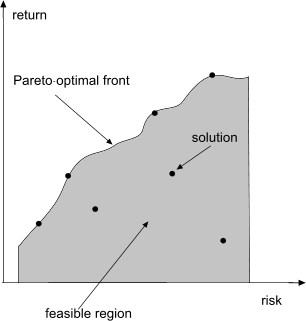
\includegraphics[scale=.9]{pareto_front.png}
  \end{center}
  \caption{Pareto-optimal front of portfolio optimization problem}
\end{figure}


Pareto-optimal front is the set of choices that are \emph{non-dominated} (\cite{drezewski2008coevolutionary}).
 

